\documentclass[solution, letterpaper]{cs121}

\usepackage{tikz-qtree}
\usepackage{graphicx}

%% Please fill in your name and collaboration statement here.
%\newcommand{\studentName}{Renzo Lucioni and Daniel Broudy}
%\newcommand{\collaborationStatement}{I collaborated with...}
\newcommand{\solncolor}{red}
\begin{document}

\header{3}{March 15, 2013, at 12:00 PM}{}{}

%%%%%%%%%%%%%%%%%%%%%%%%%%%%%%%%%%%%%%%%%%%%%%%%%%%%
\problem{20} 

%%%%%%%%%%%%%%%%%%%%%%%%%%%%%%%%%%%%%%%%%%%%%%%%%%%%
\problem{25} 

%%%%%%%%%%%%%%%%%%%%%%%%%%%%%%%%%%%%%%%%%%%%%%%%%%%%
\problem{24} 

%%%%%%%%%%%%%%%%%%%%%%%%%%%%%%%%%%%%%%%%%%%%%%%%%%%%
\problem{75}
\begin{enumerate}
	\item 
		\begin{enumerate}
			\item The requested graph is below.
				\begin{center}
				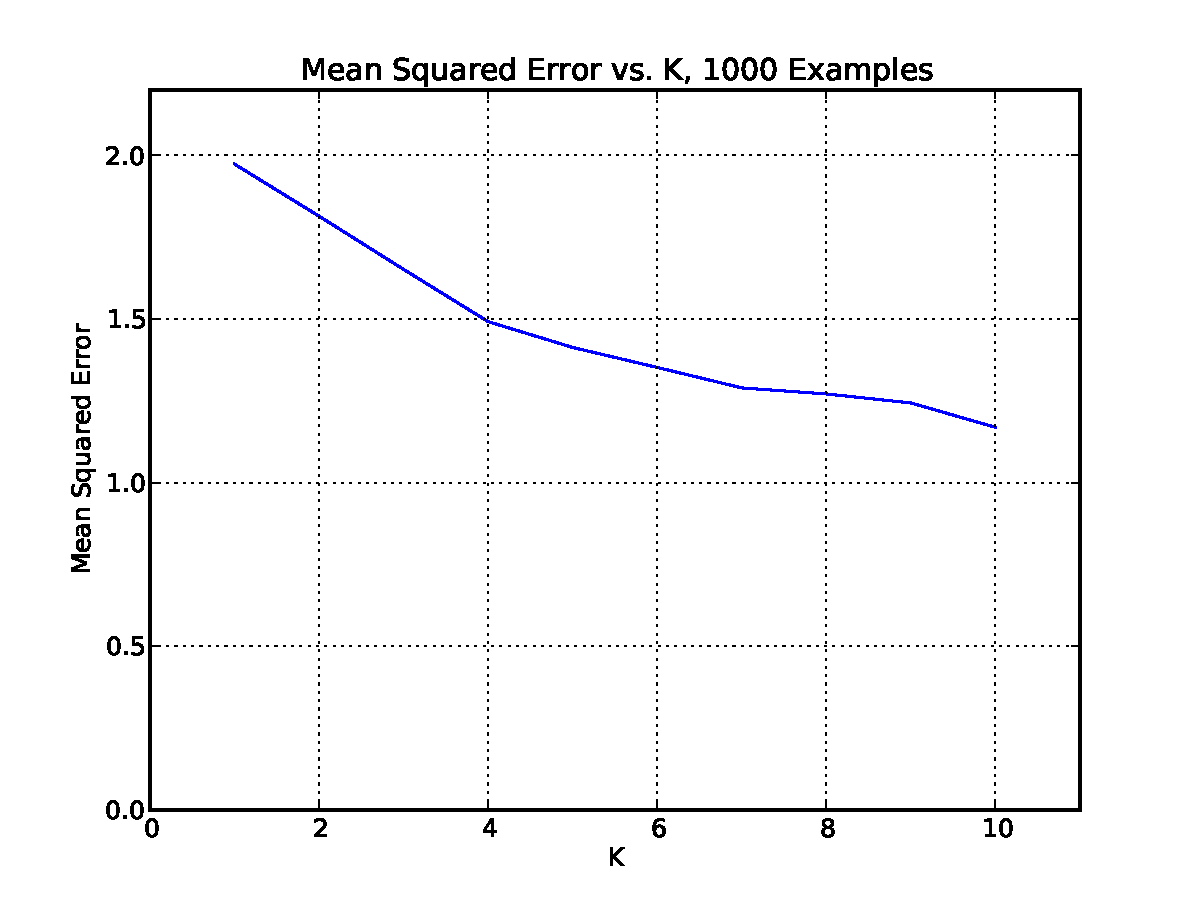
\includegraphics[scale=0.8]{mse-vs-k.pdf}
				\end{center}
			\item If we were to choose the best $K$ for this data based on the plot we generated above, we would choose $K = 8$, since this value of $K$ has a relatively low mean squared error (MSE) without the risk of overcomplicating the model. Choosing a higher value of $K$ will of course result in a lower MSE, but doing this defeats the purpose of clustering, since we are overfitting to the data. In the extreme case, every example in the data will have its own cluster, and the MSE will be 0, but this model does not generalize well.
		\end{enumerate}
	\item
	\item
\end{enumerate}

\end{document}



